\documentclass{article}

\usepackage[utf8]{inputenc}
\usepackage{comment}
\usepackage[french]{isodate}

\usepackage{graphicx}
\usepackage{siunitx}
\usepackage{paracol}
\usepackage{amsmath}
\usepackage{ amssymb }
\usepackage[utf8]{inputenc}
\usepackage[bookmarks=true]{hyperref}
\usepackage{bookmark}
\usepackage{centernot}
\usepackage{enumitem}
\usepackage{mathtools,xparse}
\usepackage{bm}


\DeclarePairedDelimiter{\abs}{\lvert}{\rvert}
\DeclarePairedDelimiter{\norm}{\lVert}{\rVert}

%Math typeset and settings
\sisetup{output-decimal-marker = {,}}
\newcommand*{\ft}[1]{_\mathrm{#1}} 
\newcommand*{\dd}{\mathop{}\!\mathrm{d}}
\newcommand*{\tran}{^{\mkern-1.5mu\mathsf{T}}}%transpose of matrix






%Math shortcuts
\newcommand{\vout}{v\ft{out}}

\begin{document}
	\begin{titlepage}
		\begin{center}
			\vspace*{1cm}
			\textbf{Math350}\\
			\text{Graph theory}\\
			\vspace{0.5cm}
			Homework II
			
			\vspace{1.5cm}
			
			\textbf{Frédéric Boileau}\\
			\vspace{2cm}
			Prof. 
			Jan Volec
			\vfill
			\today
			\thispagestyle{empty}
		\end{center}
	\end{titlepage}
	\newpage
	\pdfbookmark{\contentsname}{Contents}
	\tableofcontents
	\thispagestyle{empty}
	\clearpage
	
	\section{}
	a)
	\begin{figure}[htbp!]
		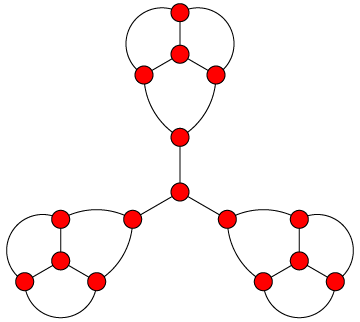
\includegraphics[width = \textwidth]{cubic-unmatchable.png}
		\caption{3-regular graph without a perfect matching}
	\end{figure}\\[2ex]
	b)
	Assume the 3-regular graph G contains a perfect matching M. Certainly then G-E(M) is a spanning connected subgraph of G. Moreover the degree of every vertex is now 2 since all the vertices were by definition adjacent to only one edge of the matching. Hence the graph contains a 2 factor. \\
	For the converse assume G is a 3-regular graph which contains a 2-factor, say F. A 2-factor is a spanning 2-regular subgraph. Consider H=G-E(F), then the degree of all vertices of H is 2. Moreover V(H) = V(G), so E(H) is a 2-regular spanning subgraph   
	
	\clearpage
	
	\section{}
	
	Every graph G contains a subgraph H that is bipartite and has at least half the number of edges of G. We proceed by induction. First assume it is true for some n. The base case is trivial. Now let G be a graph of order n+1 and $v \in V(G)$. Now consider $G' = G-v$. We have that $\abs{V(G')} = n$ so it contains a bipartite subgraph, say H, with $\abs{E(H)}\geq \abs{E(G')}/2$. Assume WLOG that H is a partition on the vertices of G' with parts A and B. Any isolated vertex can be put in either A or B. A non-isolated vertex can be put in either by removing all the edges that connects it to the opposite set. Now for the induction step we consider the removed edge v. Assume WLOG that $\abs{N_G(v) \cap  A} \geq \abs{N_G(v)\cap B}$. Now simply add all the edges linking v to vertices in A, then v is in the set B and we added at least half the edges adjacent to v, which were all the edges in G but not G', so we have constructed a bipartite subgraph with at least as many edges as contained in G. 
	\clearpage
	\section{}
	
	We want to prove that for all spanning trees ($T$) there is a corresponding even subset of the edges of G, say $F_T(G)$ such that their union gives us  the graph G. First we need to prove that the symmetric difference of two even sets is even.\\
	
	We will use the phrase  "connected by an even number of edges" even when meaning not connected, which is right as 0 is even, but we remind it just so the language stays clear:\\
	
	Consider $H = F \backslash F'$ and $K = F'\backslash F$ where both $F$ and $F'$ are even degree and consider an edge $v\in V(G)$. 
	If v connected by an even number of edges to both F and F', then is is connected by an even number of edges to H and K; if we remove an even number of edges from an even number of edges we are left with...an even number of edges. Hence H and K are even. We claim the union of two even-degree sets is still even-degree. Think of taking the union of edge sets as operations on the degrees of the vertices of one of the sets. The degrees of H are even, so adding an even number of degrees gives us a still even degree.\\
	
	\\
	
	\clearpage
	
	We want to find and even set $F_T(G)$ such that it contains at least all the edges in $E(G)\backslash E(T)$ for an arbitrary spanning tree T. Let $K = E(G)\backslash E(T)$ and $\abs K = m$. First consider the set of edges $\{e_i\} = \{u_iv_i\}$. Moreover let $P_i$ denote the unique path from $u_i$ to $v_i$ in T. Now obviously $e_i\notin P_i$. Also $e_i + P_i$ forms a cycle, thus an even set. Now consider $F_T$:
	\begin{equation}\label{biutiful}
		F_T:=\mathop\bigtriangleup_{i=1}^{m} (e_i + P_i)
	\end{equation}
	Which is the symmetric difference of all those cycles one after the other. We claim that that set contains all the edges not in the spanning tree T. TO see this we observe than we can rewrite \ref{biutiful} the following way:
	\begin{align}\label{clearly}
		F_T = \left[\mathop\bigtriangleup_{i \neq j}^{m}(e_i+P_i)\right] \quad \bigtriangleup  \quad (e_j + P_j)
	\end{align}
	We see clearly from \ref{clearly} that the if $e_j\notin F_T$ it has to be that 
	\begin{equation}\label{impossible}
		e_j \in \mathop\bigtriangleup_{i \neq j}^{m}(e_i+P_i)
	\end{equation}
	But this is impossible, to see this consider the fact that. 
	\begin{align*}\\
		\mathop\bigtriangleup_{i \neq j}^{m}(e_i+P_i) \subsetneq \bigcup_{i\neq j}^{m}(e_i + P_i) 
	\end{align*}
	Now by definition $e_j$ is not in T so cannot be in any of the $P_i$'s which are paths in the tree, also, quite trivially, $e_j$ cannot be $e_i$ if $i\neq j$. Therefore \ref{impossible} is not true. 
	
	To sum the proof up we have that \ref{impossible} is impossible, thus $F_T$ contains all the edges not in T. Moreover it is even as it is the repeated symmetric difference of even sets (cycles). QED.
	
	\clearpage
	\section{}
	
	We want to prove that for a cubic graph G the edge connectivity $\lambda(G)$ is equal to the vertex connectivity $\kappa(G)$. First if G is disconnected we have the trivial case $\kappa(G) = \lambda(G) = 0$. Now consider $\kappa(G)= 3$. Well it follows directly that the $\lambda(G) = 3$ from the fact that for all graphs $\kappa(G) \leq \lambda(G)$ with the fact that the edge connectivity of a cubic graph cannot be higher than three (we can always disconnect a graph by removing 3 edges adjacent to the same vertex). So we have two cases remaining $\bm {\kappa(G) = 1}$ (case 1) or $\bm{\kappa(G)= 2}$ (case 2). So let's consider the corresponding set of minimum edge cut, say $F$. For either case $G-U$ is disconnected by definition. Let $G_1$ and $G_2$ denote the two components of $G-F$.
	\begin{equation}\label{ineq}
		\kappa(G) \leq \lambda(G) \leq \delta(G)
	\end{equation}
	\begin{enumerate}
		\item $\abs F = 1$ which means that F consists of a cut vertex, say u. WLOG this vertex as two edges going into $G_1$ and one going into $G_2$. That last edge is a bridge and so $\lambda(G) = 1$
		\item  $\abs F = 2$. Let $F = \{u,v\}$. 
		\begin{enumerate}
			\item $uv \in E(G)$, then both u and v have exactly one neighbor in $G_1$ and $G_2$, say $u'$ and $v'$. Then $\{uu'\} $ and $\{vv'\}$ together are an edge cut. Together with \ref{ineq} means we have $\lambda(G) = 2$
			\item $uv \notin E(G)$.  Let $u'$ be the neighbor of u which is alone in one of the components of $G-F$ and analogously for $v'$. If $u'$ and $v'$ are in the same component of $G-F$ then $\{uu'\}$ and $\{vv'\}$ form and edge cut and we have with \ref{ineq} $\lambda(G) = 2$. If on the other hand $u'$ and $v'$ are not in the same component once again remove $\{uu'\}$ and $\{vv'\}$. Then WLOG $N_u \in G_1$ and $N_v \in G_2$, moreover by assumption $uv \notin G-F$ and so $\lambda(G) = 2$ which completes the proof. 
		\end{enumerate}
	\end{enumerate}
	
	
	
	\clearpage
	
		
	
	
	
	
	
	

	
	
	
	
	
\end{document}